\item Ignoring the friction between the piston and the cylinder, the correct statement(s) is(are)
        \begin{center}
            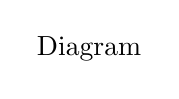
\begin{tikzpicture}
                \node at (0,0) {Diagram};
            \end{tikzpicture}
        \end{center}
        \begin{tasks}(1)
            \task If \( V_2 = 2V_1 \) and \( T_2 = 3T_1 \), then the energy stored in the spring is \( \frac{1}{4} P_1V_1 \)
            \task If \( V_2 = 2V_1 \) and \( T_2 = 3T_1 \), then the change in internal energy is \( 3P_1V_1 \)
            \task If \( V_2 = 3V_1 \) and \( T_2 = 4T_1 \), then the work done by the gas is \( \frac{7}{3} P_1V_1 \)
            \task If \( V_2 = 3V_1 \) and \( T_2 = 4T_1 \), then the heat supplied to the gas is \( \frac{17}{6} P_1V_1 \)
        \end{tasks}